\documentclass[10pt]{article}

\usepackage[top=0.8in,bottom=0.8in]{geometry}
\usepackage{amsmath}
\usepackage{amssymb}
\usepackage{enumitem}
\usepackage{graphicx}
\usepackage[T1]{fontenc}
\usepackage{array,multirow}
\usepackage[table]{xcolor}
\usepackage{tikz}
\usetikzlibrary{positioning}
\usepackage{mathtools}
% Enables font change size in verbatim blocks
\makeatletter
\newcommand{\verbatimfont}[1]{\renewcommand{\verbatim@font}{\ttfamily#1}}
\makeatother
\usepackage{hyperref}
\hypersetup{
    colorlinks=true,
    linkcolor=blue,
    filecolor=magenta,      
    urlcolor=cyan,
}
 
\urlstyle{same}

% Format for answering questions
\newenvironment{answer}
    {\begin{center}
    \begin{tabular}{|p{1\textwidth}|}
    \hline
    }
    { 
    \\\hline
    \end{tabular} 
    \end{center}
    }

% Big arrow to go between diagrams
\def\Arrow{\raisebox{-.5\height}{\scalebox{2}{$\rightarrow$}}}

\begin{document}

\title{CS 4120: Homework 2}
\author{Adam Camilli (aocamilli@wpi.edu)}
\date{\today}
\maketitle

\section*{Problem 1}
Describe a $O(n)$ time algorithm that, given a set $S$ of $n$ distinct numbers and a positive integer $k \le n$, determines the $k$ numbers in $S$ that are closest to the median of $S$. (15 points)
\begin{answer}
\begin{enumerate}
\item Find median. This takes $O(n)$ time in the worst case using the famed \href{https://tinyurl.com/yby5e74p}{median-of-medians} selection algorithm. 
\item Create an associative array $B[i][x]$ whose values are equal to the members of $S$. Let each of these values $i$ have an associated key $x$ equal to the absolute value of the difference of $i$ from the median (creation of this array is again $O(n)$):
  \begin{center}
    \begin{tabular}{|c|c|}
      \multicolumn{2}{c}{\textbf{B}} \\
      \hline
      $i_1$ & $\left| i_i - m \right|$ \\
      \hline
      $i_2$ & $\left| i_2 - m \right|$ \\
      \hline
      $\ldots$ & $\ldots$ \\
      \hline
    \end{tabular}
  \end{center}
\item Let $t$ be the $k$-th statistic selection of $B$'s key values. That is, let $t$ be equal to the $k$-th smallest element of the differences of each of $S$'s elements from the median of $S$. This calculation is once again $O(n)$ in the worst case.
\item Finally, locate the $k$ keys of $B$ with the smallest distance from the median, i.e. the $k$ keys that are less than or equal to $t$:
  \begin{center}
    \texttt{for(i=1;i<=n;i++)\\        
            \hspace{1cm}if B[i].key <= s\\           
            \hspace{3cm}print(B[i].value);\\}
  \end{center}
 The values associated with these keys are the answers. 
\end{enumerate}
\end{answer}

\newpage

\section*{Problem 2}
Write a complete pseudocode to find the predecessor of a node in a binary search tree. (10 points)
\begin{answer}
  Intuitively, a method to compute the predecessor can be described in two steps:
  \begin{enumerate}
  \item If the node has a right subtree, return its max element.
  \item Otherwise, return the highest ancestor (i.e. the one that is farthest down in tree) of the node, whose right child is also an ancestor of the node (this right child can be the node itself).
  \end{enumerate}
  A complete pseudocode to accomplish this is as follows: \\
\begin{verbatim}
predecessor (BTree tree, Node target):
    if (tree.right != NULL):
        return treeMax(tree.right);
    elif (tree.root == target):
        return NULL;
    
    Node r = tree.root;
    while (r.left != target && r != target):
        if (r.right == NULL):
            return NULL;
        r = r.right:
   
    return r;
\end{verbatim}

\end{answer}

\section*{Problem 3}
Show the red-black trees that result after successively inserting the keys 41, 38, 31, 12, 19, 8 into an initially empty red-black tree. Show all steps. (15 points)
\vspace{2cm}
\begin{center}
  {\Large(on next page)}
\end{center}
\begin{answer}
  \\
  \begin{minipage}[t]{0.3\linewidth}
    Insert 41: \\ \\
    
\begin{tikzpicture}[[level/.style={level distance=1cm, sibling distance=20mm/#1}]
      \node[inner sep=2pt,minimum size=8mm,font=\bf,fill=black,text=white,circle,draw=black](41){41}
      ;
    \end{tikzpicture}
  \end{minipage}
  \\ \\
  \begin{minipage}[t]{0.3\linewidth}
    Insert 38: \\ \\
    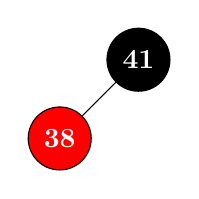
\begin{tikzpicture}[level/.style={level distance=1cm, sibling distance=20mm/#1}]
      \node[inner sep=2pt,minimum size=8mm,font=\bf,fill=black,text=white,circle,draw](41){41}
      child{
        node[inner sep=2pt,minimum size=8mm,font=\bf,fill=red,text=white,circle,draw](38){38}
      }
      child[missing]{node{}}
      ;
    \end{tikzpicture}
  \end{minipage}
  \\ \\
  \begin{minipage}[t]{0.3\linewidth}
    Insert 31: \\ \\
    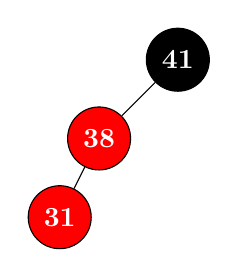
\begin{tikzpicture}[level/.style={level distance=1cm, sibling distance=20mm/#1}]
      \node[inner sep=2pt,minimum size=8mm,font=\bf,fill=black,text=white,circle,draw](41){41}
      child{
        node[inner sep=2pt,minimum size=8mm,font=\bf,fill=red,text=white,circle,draw](38){38}
        child{
          node[inner sep=2pt,minimum size=8mm,font=\bf,fill=red,text=white,circle,draw](31){31}
        }
        child[missing]{node{}}
      }
      child[missing]{node{}}
      ;
    \end{tikzpicture}
  \end{minipage}
  \begin{minipage}[c]{0.08\linewidth}
    $\Arrow$
  \end{minipage}
  \begin{minipage}[t]{0.3\linewidth}
    Case 3: Balance around 38 and recolor 38 black as root: \\ \\
    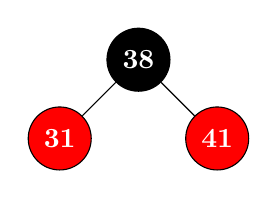
\begin{tikzpicture}[level/.style={level distance=1cm, sibling distance=20mm/#1}]
      \node[inner sep=2pt,minimum size=8mm,font=\bf,fill=black,text=white,circle,draw](38){38}
      child{
        node[inner sep=2pt,minimum size=8mm,font=\bf,fill=red,text=white,circle,draw](31){31}
      }
      child {
        node[inner sep=2pt,minimum size=8mm,font=\bf,fill=red,text=white,circle,draw](41){41}
      }
      ;
    \end{tikzpicture}
  \end{minipage}
  \\ \\
  \begin{minipage}[t]{0.3\linewidth}
    Insert 12: \\ \\
    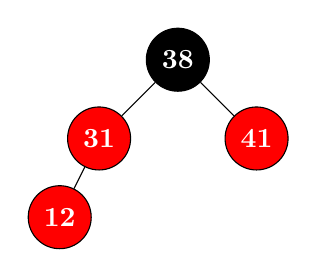
\begin{tikzpicture}[level/.style={level distance=1cm, sibling distance=20mm/#1}]
      \node[inner sep=2pt,minimum size=8mm,font=\bf,fill=black,text=white,circle,draw](38){38}
      child{
        node[inner sep=2pt,minimum size=8mm,font=\bf,fill=red,text=white,circle,draw](31){31}
        child {
          node[inner sep=2pt,minimum size=8mm,font=\bf,fill=red,text=white,circle,draw](12){12}
        }
        child[missing]{node{}}
      }
      child {
        node[inner sep=2pt,minimum size=8mm,font=\bf,fill=red,text=white,circle,draw](41){41}
      }
      ;
    \end{tikzpicture}
  \end{minipage}
  \begin{minipage}[c]{0.08\linewidth}
    $\Arrow$
  \end{minipage}
  \begin{minipage}[t]{0.3\linewidth}
    Case 1: Recolor 31 and 41. Case 0: Recolor root. \\ \\
    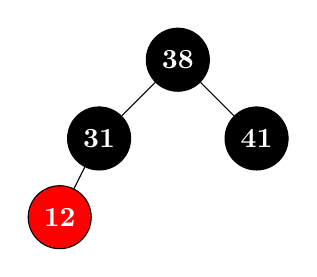
\begin{tikzpicture}[level/.style={level distance=1cm, sibling distance=20mm/#1}]
      \node[inner sep=2pt,minimum size=8mm,font=\bf,fill=black,text=white,circle,draw](38){38}
      child{
        node[inner sep=2pt,minimum size=8mm,font=\bf,fill=black,text=white,circle,draw](31){31}
        child {
          node[inner sep=2pt,minimum size=8mm,font=\bf,fill=red,text=white,circle,draw](12){12}
        }
        child[missing]{node{}}
      }
      child {
        node[inner sep=2pt,minimum size=8mm,font=\bf,fill=black,text=white,circle,draw](41){41}
      }
      ;
    \end{tikzpicture}
  \end{minipage}
  \\ \\
  \begin{minipage}[t]{0.3\linewidth}
    Insert 19: \\ \\
    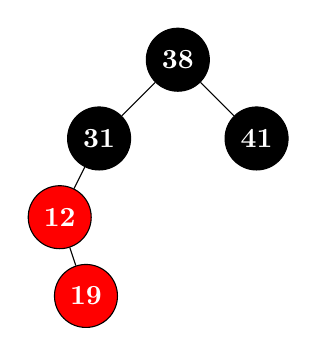
\begin{tikzpicture}[level/.style={level distance=1cm, sibling distance=20mm/#1}]
      \node[inner sep=2pt,minimum size=8mm,font=\bf,fill=black,text=white,circle,draw](38){38}
      child{
        node[inner sep=2pt,minimum size=8mm,font=\bf,fill=black,text=white,circle,draw](31){31}
        child {
          node[inner sep=2pt,minimum size=8mm,font=\bf,fill=red,text=white,circle,draw](12){12}
          child[missing]{node{}}
          child {
            node[inner sep=2pt,minimum size=8mm,font=\bf,fill=red,text=white,circle,draw](19){19}
          }
        }
        child[missing]{node{}}
      }
      child {
        node[inner sep=2pt,minimum size=8mm,font=\bf,fill=black,text=white,circle,draw](41){41}
      }
      ;
    \end{tikzpicture}
  \end{minipage}
  \begin{minipage}[c]{0.08\linewidth}
    $\Arrow$
  \end{minipage}
  \begin{minipage}[t]{0.4\linewidth}
    Case 2: Rebalance subtree around 19. Recolor 19 and 31. \\ \\
    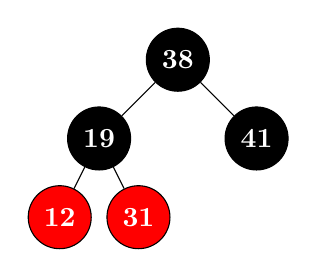
\begin{tikzpicture}[level/.style={level distance=1cm, sibling distance=20mm/#1}]
      \node[inner sep=2pt,minimum size=8mm,font=\bf,fill=black,text=white,circle,draw](38){38}
      child{
        node[inner sep=2pt,minimum size=8mm,font=\bf,fill=black,text=white,circle,draw](19){19}
        child {
          node[inner sep=2pt,minimum size=8mm,font=\bf,fill=red,text=white,circle,draw](12){12}
        }
        child {
          node[inner sep=2pt,minimum size=8mm,font=\bf,fill=red,text=white,circle,draw](31){31}
        }
      }
      child {
        node[inner sep=2pt,minimum size=8mm,font=\bf,fill=black,text=white,circle,draw](41){41}
      }
      ;
    \end{tikzpicture}
  \end{minipage}
  \\ \\
  \begin{minipage}[t]{0.31\linewidth}
    Insert 8: \\ \\
    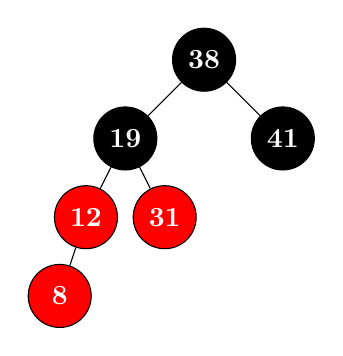
\begin{tikzpicture}[level/.style={level distance=1cm, sibling distance=20mm/#1}]
      \node[inner sep=2pt,minimum size=8mm,font=\bf,fill=black,text=white,circle,draw](38){38}
      child{
        node[inner sep=2pt,minimum size=8mm,font=\bf,fill=black,text=white,circle,draw](19){19}
        child {
          node[inner sep=2pt,minimum size=8mm,font=\bf,fill=red,text=white,circle,draw](12){12}
          child {
            node[inner sep=2pt,minimum size=8mm,font=\bf,fill=red,text=white,circle,draw](8){8}
          }
          child[missing]{node{}}
        }
        child {
          node[inner sep=2pt,minimum size=8mm,font=\bf,fill=red,text=white,circle,draw](31){31}
        }
      }
      child {
        node[inner sep=2pt,minimum size=8mm,font=\bf,fill=black,text=white,circle,draw](41){41}
      }
      ;
    \end{tikzpicture}
  \end{minipage}
  \begin{minipage}[c]{0.08\linewidth}
    $\Arrow$
  \end{minipage}
  \begin{minipage}[t]{0.31\linewidth}
    Case 1: Recolor 19, 12, and 31.  \\ \\
    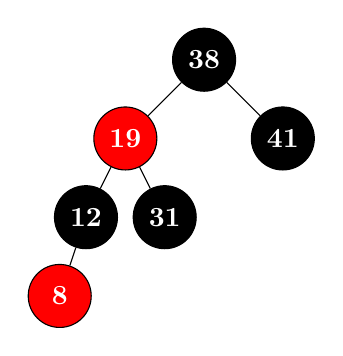
\begin{tikzpicture}[level/.style={level distance=1cm, sibling distance=20mm/#1}]
      \node[inner sep=2pt,minimum size=8mm,font=\bf,fill=black,text=white,circle,draw](38){38}
      child{
        node[inner sep=2pt,minimum size=8mm,font=\bf,fill=red,text=white,circle,draw](19){19}
        child {
          node[inner sep=2pt,minimum size=8mm,font=\bf,fill=black,text=white,circle,draw](12){12}
          child {
            node[inner sep=2pt,minimum size=8mm,font=\bf,fill=red,text=white,circle,draw](8){8}
          }
          child[missing]{node{}}
        }
        child {
          node[inner sep=2pt,minimum size=8mm,font=\bf,fill=black,text=white,circle,draw](31){31}
        }
      }
      child {
        node[inner sep=2pt,minimum size=8mm,font=\bf,fill=black,text=white,circle,draw](41){41}
      }
      ;
    \end{tikzpicture}
  \end{minipage}
  \\
\end{answer}
  
\section*{Problem 4}
Consider a connected weighted graph where the edge weights are all distinct. Show that for every cycle
of the graph, the edge of maximum weight on the cycle does not belong to any minimum spanning
tree of the graph. (15 points)

\section*{Problem 5}
A certain professor thinks that he has worked out a simpler proof of correctness for Dijkstra’s
algorithm. He claims that Dijkstra’s algorithm relaxes the edges of every shortest path in the graph in
the order in which they appear on the path, and therefore the path-relaxation property applies to every
vertex reachable from the source. Show that the professor is mistaken by constructing a directed graph
for which Dijkstra’s algorithm could relax the edges of a shortest path out of order. (15 points)

\section*{Problem 6}
In all the shortest paths algorithms we've learned in class we break ties arbitrarily. Discuss how to
modify these algorithms such that, if there are several different paths of the same length, then the one with the minimum number of edges will be chosen. (15 points)

\section*{Problem 7}
In a directed graph a set of paths is edge-disjoint if their edge sets are disjoint, i.e. no two paths share an edge (although they may share vertices). Given a directed graph $G = (V, E)$ with two distinguished vertices $s$ and $t$, give an efficient algorithm to find the maximum number of edge-disjoint $s − t$ (directed) paths in $G$. (Hint: Use a flow network.). (15 points)



\end{document}
